%!TEX root = ../main.tex
\chapter{DISEÑO Y DESARROLLO DE UN ROBOT SSL}
\label{ch:disenio_y_des}
%\includegraphics[width=\textwidth]{diagArq.png}\\

% En general: descprición general de cada sección de DyDdP. Despues, una descripción específica de cada sección del robot.
En éste capitulo se presentan los resultados del diseño de un robot \gls{SSL} de acuerdo a la metodología de \textit{Diseño y Desarrollo de Producto} \cite{ulrich2009dise}. En el primer paso, \textit{Planeación}, se establecen las restricciones del producto y los objetivos que debe cumplir. En \textit{Desarrollo de Concepto} se prueba la viabilidad del uso de ciertas tecnologías mediante prototipos, para validar el concepto. En el tercer paso, \textit{Diseño a Nivel Sistema} se establece la arquitectura del producto definiendo los sistemas y componentes que lo conforman además de identificar interacciones y las interfaces entre los sistemas. El cuarto paso \textit{Diseño a Detalle} presenta el diseño final de los componentes de cada sistema y sus características. El quinto paso, \textit{Pruebas}, se presenta como parte del capítulo \ref{ch:res}.  
\EXCISE{
	\section {Planeación}
% Capítulos: 2, 3, 4, 5, 6, 7, 8, 9, 10, 15, 16, 17, 18
% Identificación de oportunidades abarcando la evaluación de los avances tecnológicos y los objetivos.
 % El resultado es la declaración de misión del proyecto que especifica el objetivo del producto, los supuestos básicos y las limitaciones. \par
% Producto de Plataforma


El robot está enfocado en la Plataforma existente de SSL: Visión especialmente \\
Se definió la arquitectura del sistema mostrada en la Fig. \ref{fig:diagArq}. \\
La arquitectura se realizó pensando el facilitar la modularidad. Facilitando la adaptación a otras aplicaciones así como poder modernizar por módulos cuando sea necesario. \\
Debido a que el robot, aunque independiente del sistema con el que se utilice, se valida con un sistema en específico (Robocup SSL), es importante incluir éste sistema dentro de la arquitectura. \\

\begin{figure}
	\centering
		\includegraphics[width=8cm]{diagArq.png}
	\caption{Arquitectura del Robot}
	\label{fig:diagArq}
\end{figure}
}
\EXCISE{
\subsection {Movimiento}
Se requiere movimiento omnidireccional para poder estar a la par de las capacidades de todos los equipos de Robocup SSL. \\
Para el movimiento omnidireccional, es necesario una rueda omnidireccional. \\
Es necesaria una rueda delgada \\
Rueda comercial: Mecanum, pero son muy anchas para esta aplicación \\
Es necesario diseñar y manufacturar una rueda propia que cumpla con las necesidades\\

\subsection {Pateo}
Existen dos tipos de pateo permitidos en SSL: straight y chip \\
Actualmente todos los equipos cuentan con ambos tipos de pateo \\
Dos posibilidades: neumático y eléctrico \\
El eléctrico ocupa menos espacio y se puede utilizar más veces sin recargar: aprendido de los TDP's de otros equipos \\
Son necesarios dos selenoides y un circuito de carga (con capacitor) que se autoregule \\
Dos tipos de Selenoides: comerciales y hechos en casa? \\
Se utiliza comercial por ser más eficiente aunque se pierde posibilidad de no ser cilíndrico y adaptarlo al espacio del robot \\
Se utiliza un sistema de palanca para poder tener un chip kicker \\
La primera generación de Eagle Knights con chip kicker \\

\subsection {Control de Pelota}
Es necesario para realizar un pateo eficiente \\
Escencial para mover la pelota cerca del robot \\
Por especificaciones de SSL, tiene que ser parelo al suelo \\
Los diseños de otros equipos utilizan motores brush con algún tipo de transmisión \\
Para el dribbler, se utilizan diversos tipos de espongas, material suaves \\

\subsection {Electrónica - Circuitos}
Se puede utilizar: FPGA, Microcontrolador, DSP, Computadora miniatura (Raspebbry Pi) y combinaciones \\

\subsection {Comunicación}
SSL permite cualquier tipo de comunicación inalámbrica excepto Bluetooth \\
Entre las opciones más populares estan: \gls{Wi-Fi}, Xbee, radios en otras frecuencias \\

\subsection {Energía}
Es necesario alimentar: Movimiento, Electrónica - Circuitos, Pateo, Comunicación \\



\subsection {ROS}
Debido a que se busca favorecer la modularidad en la totalidad del sistema, se decidió utilizar ROS \\
ROS se basa en módulos que se comunican entre sí, facilitando la escalabilidad y mejoramiento del sistema y los subsistemas. \\
}

% \subsection {Diseño}
% Considerar Plataforma y Arquitectura. \par
% Evaluar Nuevas Tecnologías. \par
% \subsection {Manufactura}
% Identificar restricciones de producción. \par
% Establecer estrategia para la Cadena de Suministro \par
% \subsection {Otras} 
% Investigación: Demostrar Tecnologías \par
% Dirección Gral: Asignar Recursos \par

\section {Planeación}

% Capítulos: 2, 5, 6, 7, 8, 9, 10, 11, 12, 14, 15, 16, 17, 18
% Se identifican las necesades del mercado objetivo
% se generan y evalúan conceptos alternativos del producto 
% uno o más conceptos se seleccionan para desarrollar
% pruebas adicionales, 
Se hace la planeación considerando las características de versiones previas y las especificaiones de la \gls{SSL}.
Las características de versiones anteriores del Robot para Robocup \gls{SSL} que se toman en cuenta en este diseño son:
\begin{itemize}
	\item Alta dependencia de manufactura externa, por no contar con el equipo necesario para realizar manufactura interna.
	% \item Alta dependencia de manufactura externa.\par Esto representa dificultad para realizar prototipaje además de elevar costos.
	\item Piezas frágiles, requiriendo ser reemplazadas frecuentemente durante pruebas y juegos. La rueda era uno de los componentes con mayores problemas.
	% \item Piezas frágiles. \par Se necesitaba reemplazar con alta frecuencia ciertas piezas, elevando costos.
	\item Tiempo de ensamblado elevado debido al número de piezas, impactando en los costos.
	% \item Tiempo de armado elevado. \par Producto de un elevado número de piezas únicas, además de elevar costos por requerir mayor material y manufactura.
	% \item Muchas piezas comerciales. \par Alta dependencia de terceros además de elevar los costos.
	% \item Difícilmente modificable. \par Una pieza cumplía múltiples funciones.
	\item Cómputo basado en un \gls{DSP} volviendo la programación compleja, difícil de parametrizar y modificar.
	\item No se tenía un diseño modular, haciendo difícil realizar modificaciones. 
	\item La carcasa no tenía el \gls{SP} integrado en su diseño, presentando problemas con la visión de la liga y siendo complejo modificar el \textit{id} de cada robot.
	\item Problemas en el sistema de energía, afectando particularmente a los motores. Estos requerían ser reemplazados frecuentemente tras descomponerse. Además de elevar costos, el tiempo de reemplazo era alto.

	% \item Mala integración con la visión de la liga. \par Las carcasas no se realizaban con un método de manufactura automatizado, provocando teniendo alto margen de error y problemas con el reconocimiento de cada robot por el sistema de visión de la liga.
\end{itemize}


En la sección \ref{robocup-ssl} se detallan las reglas y especificaciones que un robot debe cumplir para poder participar en Robocup \gls{SSL}. La solución debe cumplir con dichas especificaciones además de atacar los problemas detectados en versiones anteriores. Específicamente, el robot debe ser fácilmente modificable y de bajo costo, priorizando manufactura local.

Para poder mantener bajos costos y asumiendo que se tendrá una producción de pocas unidades, el método de \gls{MDF} resulta muy atractivo al contar en el laboratorio con el equipo adecuado. A pesar de ésto, no se pueden descartar otros métodos de manufactura ni utilizar piezas comerciales al proporcionar mayor calidad.


\section{Desarrollo de Concepto}
Para validar la viabilidad de utilizar \gls{MDF} como principal técnica de manufactura, se crearon dos prototipos utilizando piezas de versiones anteriores.

El primer prototipo se muestra en la Fig. \ref{fig:protoRob}). Tanto la base como la carcasa de cada motor se manufacturaron mediante \gls{MDF}. Mediante éste prototipo se validó la posibilidad de imprimir piezas de dimensiones similares a la base (150 mm de radio por 5mm de ancho). Aunque la base salió ligeramente dañada del proceso de \gls{MDF} por su tamaño, no afectó gravemente su estructura. Adicionalmente, con éste prototipo se pudo comenzar a probar el funcionamiento de los motores y el movimiento omnidireccional. Las ruedas utilizadas en el prototipo ocupan mucho espacio por lo que es necesario utilizar otras ruedas que ocupen menos espacio así como implementar un reductor de velocidad ya que se requiere menor velocidad de los motores y mayor torque. Por último, el motor debe ir elevado ya que de quedar cerca del suelo puede dañarse por la pelusa de la cancha.

El segundo prototipo se muestra en la Fig. \ref{fig:protoKicker}. El objetivo de éste prototipo fue validar si las piezas manufacturadas mediante \gls{MDF} se podían utilizar para el \gls{Kicker} sin que se dañasen rápidamente. Adicionalmente, se probó una primera versión del circuito de control. Las piezas funcionaron adecuadamente aunque la sujeción de las piezas presentó problemas debido a la fuerza ejercida por el selenoide.


\begin{figure}
	\centering
		\includegraphics[width=8cm]{proto_4}
	\caption{Prototipo del Robot}
	\label{fig:protoRob}
\end{figure}

\begin{figure}
	\centering
		\includegraphics[width=8cm]{proto_kicker_1}
	\caption{Prototipo del Kicker}
	\label{fig:protoKicker}
\end{figure}


\EXCISE{
	\subsection {Diseño}
	Investigar factibilidad de conceptos del producto \par
	Desarrollar conceptos de diseño industrial \par
	Construir y probar prototipos \par
	\subsection {Manufactura}
	Estimar costos \par
	Evaluar factibilidad de producción \par
	\subsection {Otras}
	Recabar necesidades \par
	Identificar Usuarios \par
	Identificar productos de la competencia \par
}
\section {Diseño a Nivel de Sistema}
% Capítulos: 2, 6, 10, 11, 12, 13, 14, 15, 16, 17, 18 
% Definir la arquitectura del producto 
% la descomposición del producto en subsistemas y componentes.
% Planes iniciales para el sistema de producción así como esquema de ensamble final para el sistema de producción. 
% Al final de esta fase se debe contar con:
	% un diseño geométrico del producto
	% una especificación funcional de cada uno de los subsistemas del producto
	% un diagrama de flujo preliminar del proceso para el ensamble final. 
% \EXCISE{
% 	\subsection {Diseño}
% 	Generar arquitecturas de producto. \par
% 	Definir subsistemas e interfaces principales. \par
% 	Refinar diseño industrial. \par
% 	Ingeniería preliminar de componentes. \par
% 	\subsection {Manufactura}
% 	Identificar proveedores para componentes clave. \par
% 	Efectuar análisis de fabricar contra comprar. \par
% 	Definir esquema final de ensamble. \par
% 	\subsection {Otras}
% 	Análisis de fabricar vs comprar \par
% }

Para realizar el Diseño a Nivel de Sistema, se identifican componentes funcionales que requiere la solución y se identifican las relaciones entre ellos para definir sistemas. Se presentan las interacciones incidentales entre los sistemas así como las interfaces entre sistemas. La arquitectura propuesta es modular, compuesta de seis sistemas.

% Se presenta una arquitectura modular con una funcionalidad específica para cada sistema que la compone: Chasis, Cómputo, Electrónica, Mecánica y Aditamentos para el Juego. \TODO{Cambiar...}

\subsection{Análisis de los Componentes del Robot}

%%%%%%%%%%%%%%%%%%%%%%%%%%%%%% BEGIN FIGURE %%%%%%%%%%%%%%%%%%%%%%%%%%%%%%
\begin{figure}
	\centering
		\includegraphics[width=\textwidth]{EKbot_Schematic.png}
	\caption{Esquemático: Elementos del Robot Omnidireccional}
	\label{fig:ekbot_schematic}
\end{figure}
%%%%%%%%%%%%%%%%%%%%%%%%%%%%%% END FIGURE %%%%%%%%%%%%%%%%%%%%%%%%%%%%%%
Para obtener una arquitectura modular, se identificaron 20 componentes necesarios de acuerdo a su función y se agruparon en 6 sistemas como se muestra en la Fig. \ref{fig:ekbot_schematic}, de los cuales dos son considerados críticos: Cómputo y Mecánica. 

\subsubsection{Chasis}
Componentes cuya función principal es proporcionar soporte estructural, protegiendo al resto de los sistemas ante colisiones. Está integrado por tres componentes: Base, Carcasa y Tapa. La función de la base es unir los sistemas mientras que la carcasa protege a los sistemas ante colisiones. La tapa implementa el \gls{SP} para ser compatible con los requerimientos de Robocup \gls{SSL}.

\subsubsection{Movimiento}
Sistema integrado por los componentes que le proporcionan movimiento en el mundo al robot. Está integrado por tres componentes: Actuador, Transmisión y Rueda. El actuador genera movimiento que se transmite mediante la transmisión a la rueda. Para obtener movimiento omnidireccional son necesarios por lo menos tres instancias de cada componente, por redundancia se utilizan cuatro. Por la funcionalidad que éste sistema proporciona es considerado crítico.

\subsubsection{Aditamentos de Apoyo}
Estos componentes son específicos para participar en juegos de Robocup \gls{SSL}. Un actuador, transmisión y rodillo son para el \gls{Dribbler} que retiene la pelota mientras que los otros dos sirven para patear la pelota. Para utilizar el robot en un contexto distinto a \gls{SSL}, éste es el sistema que se puede reemplazar.

\subsubsection{Energía}
Fuentes de corriente directa que alimentan a otros sistemas. Tanto el sistema de Movimiento como el de Aditamentos de Apoyo requieren 12V. El sistema de Cómputo requiere 5V.

\subsubsection{Drivers}
Componentes que sirven como interfaces entre sistemas. Se tienen 3 drivers, uno para cada tipo de actuador.

\subsubsection{Cómputo}
Los componentes del sistema se encargan de obtener, almacenar y procesar datos para generar y enviar señales de control a otros sistemas. Está compuesto de cinco componentes: Interfaz de Entradas/Salidas, Comunicación Inalámbrica, Función de Control, Velocímetro y Registros. El primero, sirve para comunicar componentes a través de distintos tipos de señales y protocolos de comunicación. La comunicación inalámbrica recibe datos de un sistema externo. La función de control calcula a partir de la información disponible la siguiente señal de control que aplicar a los actuadores del sistema mecánico. El velocímetro determina la velocidad real del robot mientras que la \gls{RAM} recibe datos de diversos componentes, los almacena y envía conforme son solicitados.

Se considera un sistema crítico debido a que el desempeño del robot está directamente relacionado a la frecuencia con la que éste sistema opere.





% \begin{enumerate}
% 	\item Chasis \par
% 		Componentes encargados de proporcionar soporte estructural, protegiendo al resto de los sistemas ante colisiones.
% 	\item Baterías \par
% 		Fuentes de corriente directa que alimentan a otros sistemas.
% 	\item Cómputo \par
% 		Obtener, almacenar y procesar datos para generar y enviar señales de control. 
% 	\item Drivers  \par
% 		Interfaces entre dos sistemas.
% 	\item Mecánica \par
% 		Integrado por los componentes que permiten el movimiento del robot en el mundo. 
% 	\item Aditamentos para el Juego \par
% 		Componentes específicos para participar en juegos de Robocup \gls{SSL}. 
% \end{enumerate}

\subsection{Interacciones entre Sistemas}
En la Fig. \ref{fig:incid_inter} se muestran las tres interacciones incidentales identificadas entre los distintos sistemas. La primera se da entre el chasis y los drivers, el calor generado por los drivers no se disipa rápidamente. La segunda es entre el chasis y las vibraciones generadas por la mecánica. La tercera se da al activar los componentes para el juego con la mecánica, pudiendo introducir errores en el movimiento del robot. 

Las interfaces entre los sistemas se muestran en la Fig. \ref{fig:interfaces_diag}. El sistema de baterías alimenta directamente al cómputo y a los drivers. El cómputo recibe señales del sistema mecánico y saca señales de control a los drivers que activan tanto el sistema mecánico como los aditamentos para el juego.
% A partir de la arquitectura, se realizó un análisis de las interacciones incidentales que pueden existir entre los distintos sistemas, mostrada en la Fig. \ref{fig:incid_inter}. Se identificaron tres interacciones incidentales. La primera es por el calor generado por la electrónica, especialmente por el circuito del kicker, con la carcasa al no permitir ventilación. La segunda se da por la vibración generada por los motores y ruedas, pudiendo afectar al chasis. La tercera interacción incidental se daría al activar la patada por la tercera ley de Newton. \par
% Adicionalmente, en la Fig. \ref{fig:interfaces_diag} se muestran las 3 interacciones deseadas entre los sistemas. La primera, entre Movimiento y Cómputo es bidireccional: se requiere de retroalimentación de Movimiento a Cómputo y de señales de control de Cómputo a Movimiento. La segunda se da del Computo a la Electrónica mediante señales de activación. La tercera se da de la Electrónica a los Aditamentos para la Pelota mediante señales eléctricas. \par
% Para el correcto funcionamiento del robot, son dos los sistemas críticos: movimiento y cómputo. El primero debido a que es el sistema que provee la característica omnidireccional al robot, mientras que el segundo es esencial para controlar eficazmente el movimiento del robot. Debido a ser sistemas críticos, un alto porcentaje del costo del robot debe pertenecer a estos. Como se busca crear un diseño de bajo costo, es en los otros sistemas que se debe buscar reducir el costo del robot. \par
\subsection{Arquitectura Propuesta}
En la Fig. \ref{fig:arq_rob} se muestra la arquitectura propuesta con los sistemas mencionados previamente así como los componentes de cada sistema y las interacciones existentes entre los componentes. A partir de los componentes de cada sistema, se puede comenzar a realizar el diseño a detalle de cada componente. Cada uno puede consistir de una o más piezas.


\begin{figure}
	\centering
		\includegraphics[width=\textwidth]{incidental_interactions}
	\caption{Interacciones Incidentales}
	\label{fig:incid_inter}
\end{figure}

\begin{figure}
	\centering
		\includegraphics[width=\textwidth]{Interfaces_interactions}
	\caption{Interacciones Deseadas}
	\label{fig:interfaces_diag}
\end{figure}

\begin{sidewaysfigure}
	\centering
		\includegraphics[width=\textwidth]{Arquitectura_ekbot.pdf}
	\caption{Arquitectura del Robot}
	\label{fig:arq_rob}
\end{sidewaysfigure}
% incidental_interactions  Interfaces_interactions Arquitectura_ekbot


\section{Diseño a Detalle}
% Capítulos: 11, 12, 13, 14, 15, 16, 17, 18
% Especificación completa de la geometría, materiales y tolerancias de todas las partes únicas del producto
% identificar las partes estandar a ser adquiridas de proveedores
% Al finalizar se debe contar con: 
	% documentación de control del producto: 
		% dibujos o archivos de la geometría de cada pieza
		% Especificaciones de piezas compradas
		% planes de proceso para la fabircación y ensamble del producto
% Terminar de definir: 
	% Selección de materiales
	% Costo de producción
	% Desempeño robusto del producto

En ésta sección se presentan los diseños finales obtenidos para cada componente de la arquitectura propuesta. Cada uno de los componentes son ensamblados con tornillos m3 de 5mm o 13mm de acuerdo a cada pieza. Cada componente puede estar compuesto por una o más piezas únicas. Con la finalidad de reducir costos, se prioriza utilizar como método de fabricación \gls{MDF} debido a que se cuenta con el equipo necesario. Para ello, se prioriza utilizar plástico \gls{ABS} por ser el de menor costo para ser usado en \gls{MDF} aunque se utiliza plástico \gls{HIPS} en las piezas de mayores dimensiones y que requieren mayor resistencia. Se utilizan piezas comerciales en los componentes donde se requiere alta precisión. El principal criterio de selección entre las alternativas de piezas comerciales es el costo, a menos que se trate de un sistema crítico, entonces se consideran otras características.

 % Para las piezas que necesiten ser comerciales, el principal criterio de selección es el precio a menos que pertenezcan a un sistema crítico, entonces se consideran otras características.
 % \TODO{Checar}
% Todas las piezas se pueden consutlar en \TODO{agregar liga}.

%%%%%%%%%%%%%%%%%%%%%%		CHASIS		%%%%%%%%%%%%%%%%%%%%%%
\subsection{Chasis}
Las piezas que comprenden éste sistema son las de mayores dimensiones, presentando dificultades para su manufactura por las características de dilatación del plástico \gls{ABS}. Para disminuir los problemas relacionados a manufacturar piezas grandes mediante \gls{MDF}, se utiliza plástico \gls{HIPS}. Aunque el plástico \gls{HIPS} tiene un costo superior al \gls{ABS}, se caracteriza por ser resistente a impactos, una característica deseada en la carcasa. Adicionalmente, permite manufacturar piezas de dimensiones mayores mediante \gls{MDF}, eliminando la necesidad de dividir las piezas en más pequeñas, facilitando el ensamblado. El modelo \gls{CAD} del sistema se muestra en la Fig. \ref{fig:chasis_cad}. 
% \TODO{checar, agregar total de piezas únicas}


\begin{figure}
	\centering
		\includegraphics[width=0.6\textwidth]{chassis_CAD}
	\caption{Chasis: Modelo CAD}
	\label{fig:chasis_cad}
\end{figure}
% \TODO{imagen del chasis real y cad}
\subsubsection{Tapa} 
La tapa consta de tres piezas únicas: dos diseños propios y tres imanes iguales con los que se ajusta al chasis facilitando el acceso a los componentes interiores. Una pieza cuenta con el \gls{SP}, lo cual facilita intercambiar los identificadores de cada robot. 

\subsubsection{Carcasa}
Compuesta de dos piezas únicas, su función principal es proteger al resto de los componentes ante posibles colisiones durante el juego y las pruebas. Una pieza se coloca al frente del robot, de la otra se utilizan tres y se colocan alrededor del robot ensambladas a la base. Se cuenta con orificios en las piezas para facilitar la ventilación para disipar el calor generado por los drivers.

\subsubsection{Base}
A ésta pieza se acoplan los demás sistemas así como la carcasa. Estructuralmente es una de las piezas críticas porque es el soporte de todos los componentes físicos.

\subsection{Energía}
Se utilizan dos modelos de baterías \textit{LiPo} distintas. Una batería de 7V para alimentar los componentes del Cómputo y al controlador del \gls{Dribbler}. Dos baterías de 12V alimentan a un controlador cada una. Específicamente, una alimenta a los drivers de los motores y la otra al controlador del \gls{Kicker}. El conector de la batería de 7V es distinto al de las baterías de 12V para evitar conectarlas a los sistemas erróneos. Utilizando una batería de 900mAh para la alimentación de los motores, el mínimo tiempo de uso esperado es de 6.75 minutos si los motores se encuentran a la máxima velocidad. El tiempo es el mismo para el \gls{Kicker} si el consumo de éste fuera el máximo de manera continua. 




%%%%%%%%%%%%%%%%%%%%%%%  Mecánica   %%%%%%%%%%%%%%%%%%%%%%%%%%%
\subsection{Movimiento}
El sistema mecánico está conformado por tres componentes, requiriendo cuatro \textit{instancias} de cada componente. Todas las piezas no comerciales están manufacturadas mediante \gls{MDF} utilizando plástico \gls{ABS} para reducir costos.
% \TODO{Agregar imagen del sistema cad y real}

\subsubsection{Motor}
Se utiliza un motor sin escobillas Maxon 200142 \cite{maxon_motor} que cuenta con tres sensores hall. El motor se acopla al chasis mediante una pieza propia. Motores de ésta marca han sido utilizados ampliamente por otros equipos de \gls{SSL} ya sea éste modelo o similares; estos motores habían sido previamente adquiridos para una generación anterior de los robots pero no fueron utilizados. Con la finalidad de reducir costos, se optó por utilizar estos motores en lugar de comprar nuevos. Los motores constituyen el componente más caro del robot (por necesitar cuatro) pero a la vez son uno de los componentes críticos ya que se requiere de motores eficientes, de tamaño reducido y que cuenten con retroalimentación para realizar control a lazo cerrado. En la Fig. \ref{fig:mot_trans_cad} se muestran acoplados éste componente y la transmisión.

\begin{figure}
	\centering
		\includegraphics[width=0.6\textwidth]{motor_trans_CAD}
	\caption{Motor y Transmisión: Modelo CAD}
	\label{fig:mot_trans_cad}
\end{figure}


\subsubsection{Transmisión}
Para acoplar el motor a la rueda se utiliza un tren de engranes rectos con reducción de velocidad de 3.5. Se optó por utilizar piezas comerciales debido a que se trata de un componente que requiere alta precisión para un acoplamiento adecuado. Se utilizan engranes rectos ya que, aunque éste tipo de engrane ocupa mayor espacio respecto a engranes planetarios, son más baratos. Al motor se acopla mediante un prisionero el \textit{pinion} \cite{pinion}. La rueda se acopla a un \textit{hub} \cite{dual_ball_bearing} al cual también se acopla el engrane \cite{gear_motor}.  Se utiliza como eje un tornillo de $\frac{1}{4}^{\prime\prime}$ el cual se introduce en el \textit{hub} y en \textit{motor\_hub}. Son necesarios dos separadores para ajustar la rueda a la altura del eje adecuada.

\subsubsection{Rueda}
La rueda consiste en cuatro piezas únicas: la silueta, rodillo, o-ring \cite{o-rings} y un cable. La silueta  (Fig. \ref{fig:ruedaOmni} \subref{rueda_silueta}) es la pieza principal de la rueda, está manufacturada mediante \gls{MDF}. Se utilizan 21 rodillos a los cuales se les coloca un o-ring a cada uno. Mediante el cable, se insertan los rodillos a la silueta.
En la Fig. \ref{fig:ruedaOmni} \subref{rueda_cad} se muestra el ensamble en CAD de la rueda. 
En la Fig. \ref{fig:ruedaOmni} \subref{exploded_assembly} se muestran las 4 piezas únicas utilizadas en la rueda, en orden descendiente: o-ring, rodillo, cable y silueta.

% \TODO{Agregar imagen de todo el sistema}
\begin{figure}%
	\centering
		\subfloat[Diagrama de la silueta]{{ 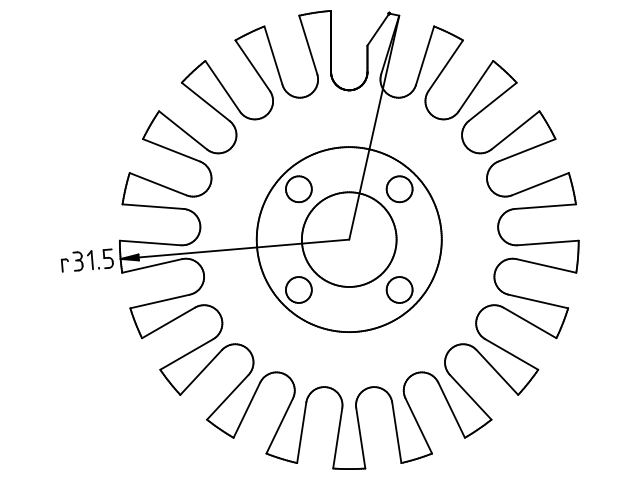
\includegraphics[width=0.4\textwidth]{rueda.png} \label{rueda_silueta} }}%
		\qquad
		\subfloat[Modelo CAD del componente]{{\includegraphics[width=0.3\textwidth]{rueda_CAD.png} \label{rueda_cad} }}%
		\qquad
		\subfloat[Piezas que conforman la rueda]{{\includegraphics[width=0.4\textwidth]{ruedaAssembly.png} \label{exploded_assembly} }}%
		\qquad
	\caption{Rueda Omnidireccional Utilizada}
	\label{fig:ruedaOmni}%
\end{figure}

%%%%%%%%%%%%%%%%%%%%%%%%%%%   ADITAMENTOS   %%%%%%%%%%%%%%%%%%%%%%%%%%%
\subsection{Aditamentos de Apoyo}
Este sistema es específico para participar en juegos de Robocup \gls{SSL}. Éste sistema se puede reemplazar si el robot es utilizado para otra aplicación.
El sistema está compuesto de cinco componentes, agrupados en dos subsistemas: \gls{Dribbler} y \gls{Kicker}. Los únicos componentes comerciales son actuadores: un motor con escobillas para el \gls{Dribbler} mientras que para el \gls{Kicker} es necesario utilizar selenoides comerciales. Para ambos casos el precio fue el principal factor de selección.

\subsubsection{Kicker}
El objetivo de éste componente es patear la pelota.
Se utiliza un selenoide como componente principal y un total de cuatro piezas únicas manufacturadas mediante \gls{MDF} para acoplar el componente al chasis. Otra pieza se acopla al selenoide para realizar el pateo de la pelota.
En la Fig. \ref{fig:cad_kicker} se muestra el modelo \gls{CAD} del kicker.

\begin{figure}
	\centering
		\includegraphics[width=0.5\textwidth]{kicker_assembly}
	\caption{Kicker: Modelo CAD}
	\label{fig:cad_kicker}
\end{figure}

\subsubsection{Dribbler}

El dribbler permite mantener al robot mantener la posesión de la pelota.
Está compuesto de tres subcomponentes: motor, transmisión y rodillo. Se utiliza un motor con escobillas \cite{dribbler_motor} debido a que no se requiere un control preciso de velocidad. Como transmisión se utiliza un tren de dos engranes manufacturados mediante \gls{MDF} debido al bajo torque que se requiere. En la Fig. \ref{fig:dribbler_cad} se muestra el modelo \gls{CAD} de éste componente así como el componente acoplado al robot.

\begin{figure}
	\centering
		\subfloat[Modelo CAD]{{ \includegraphics[width=0.4\textwidth]{dribbler_CAD} }}
		\qquad
		\subfloat[Acoplado al robot]{{ \includegraphics[width=0.4\textwidth]{dribbler_real} }}%
		\qquad	
	\caption{Dribbler}
	\label{fig:dribbler_cad}
\end{figure}


%%%%%%%%%%%%%%%%%%%%%%%%%%%   DRIVERS   %%%%%%%%%%%%%%%%%%%%%%%%%%%
\subsection{Drivers}
Éste sistema es la interfaz entre el sistema de cómputo y los actuadores. Es necesaria una interfaz debido a que el cómputo utiliza baja potencia mientras que los actuadores utilizan alta potencia. La mayoría de las piezas utilizadas en éste sistema son comerciales al tratarse de componentes eléctricos. Además de priorizar la reutilización de componentes se quiere minimizar el costo. El sistema también cuenta con piezas no comerciales manufacturadas con \gls{ABS}. La función de éstas piezas es de acoplamiento.

\subsubsection{Controlador de Motores}
Como interfaz entre el subsistema de \textit{Cómputo} y los motores sin escobillas que actuan las ruedas, se utilizan un \gls{ESC} \cite{esc_afro} por motor. Cada \gls{ESC} recibe una señal \gls{PWM} que codifica la velocidad deseada a 50 Hz, el ancho del pulso va de 1ms a 2ms, siendo 1.5ms la posición neutral. 

\subsubsection{Controlador Kicker}
El circuito está compuesto de cuatro subsecciones: carga, almacenamiento, detección de la pelota y activación. La carga se encarga de incrementar 12 V de voltaje de entrada a 200 V y mantenerlos, pasándolos al almacenamiento que consiste en un capacitor de 1000 $\mu F$. La detección de la pelota consiste en un diodo infrarrojo y un fotodiodo que activan un relevador si se detecta un objeto entre ambos. La subsección de activación recibe la señal de la \gls{FPGA}, estando aislada eléctricamente mediante octocopladores. El circuito se muestra en la Fig. \ref{fig:circuito_kicker}.

\begin{figure}
	\centering
		\includegraphics[width=\textwidth]{circuito_kicker}
	\caption{Circuito para el Kicker}
	\label{fig:circuito_kicker}
\end{figure}



\subsubsection{Controlador Dribbler}
El controlador del \gls{Dribbler} utiliza un puente H \cite{instruments2005l293} para dar energía al motor además de un regulador de voltaje que entrega 5 V a la salida. 


%%%%%%%%%%%%%%%%%%%%%%%%% Cómputo %%%%%%%%%%%%%%%%%%%%%%%%
\subsection{Cómputo}
Está compuesto por un XBee WiFi y una tarjeta de desarrollo \textit{Mojo} \cite{embedded_micro} la cual integra una \gls{FPGA} y un microcontrolador \gls{AVR}. 

% \NOTE{se podría agregar imágen de interacciones e interfacez entre Cómputo con electrónica}
% \subsubsection{\gls{FPGA} }
En la Fig. \ref{fig:arq_fpga} se muestra la arquitectura implementada en la FPGA así como los protocolos de comunicación usados entre la FPGA y los otros componentes. Los procesos implementados en la FPGA buscan aprovechar la alta frecuencia a la cual opera. Además, al no ser secuencial se pueden tener el número necesario de entradas y salidas operando de forma simultánea. En cambio, utilizar un mictrocontrolador \gls{AVR} facilita la implementación de las operaciones necesarias para realizar algoritmos de control así como realizar cálculos matriciales.
Aunque la tarjeta \textit{Mojo} representa un alto porcentaje del costo, al tener integradas una \gls{FPGA} y un \gls{AVR} ofrece características que son de gran utilidad como el manejo en paralelo de múltiples entradas y salidas. 

\begin{figure}
	\centering
		\includegraphics[width=\textwidth]{FPGA_model}
	\caption{Modelo Implementado en la FPGA}
	\label{fig:arq_fpga}
\end{figure}
% \TODO{agregar la parte de AVR ???}
\subsubsection{Comunicación Inalámbrica}

Para la comunicación inalámbrica se utiliza un XBee \gls{Wi-Fi} el cual recibe el vector $(X, Y, \theta)$ de velocidad deseada del robot además de comandos para los aditamentos. Se utiliza direccionamiento estático y mensajes UDP para evitar retransmisiones. Cada mensaje utiliza 12 bytes que codifican el vector velocidad del robot $(X, Y, \theta)$ y la acción deseada para los aditamentos de apoyo.
% Componente encargado de interactuar con el sistema externo. Recibe un vector $(X, Y, \theta )$ además del comando para los aditamentos. Los datos se los pasa al subcomponente \textit{Cómputo}. Esta compuesto por una targeta Xbee \gls{Wi-Fi} \cite{xbee_wifi}. Los datos son recibido mediante el protocolo UDP ya que solamente se requiere el último dato disponible y se evitan retransmiciones en caso de pérdida de los paquetes.

\subsubsection{Interfaz de Entrada/Salida}

Se tiene tres posibles fuentes de entrada: la comunicación inalámbrica, sensores hall de los motores y el \gls{AVR}. Para la comunicación inalámbrica es necesaria una interfaz \gls{UART} mientras que para el \gls{AVR} se utiliza una interfaz \gls{SPI}. Se utiliza una cola para guardar los datos provenientes del AVR y otra para los de la comunicación inalámbrica. Las señales de los sensores Hall se pasan al velocímetro. 

Existen cinco salidas a distintos componentes. Para la salida al \gls{AVR} se utiliza la interfaz \gls{SPI} y para la comunicación inalámbrica la interfaz \gls{UART}. Tanto para la salida a los drivers de motores como del \gls{Dribbler} se utiliza un módulo que convierte el dato a una señal \gls{PWM}. Por último, la salida al controlador del \gls{Kicker} es binaria.

% Para las salidas, se tiene una máquina de estados que de acuerdo a prioridades previamente asignadas, lee de los registros para establecer la señal adecuada en cada salida. La prioridad más alta la tiene el \gls{AVR}, la segunda el controlador de los motores, después los drivers de kicker y dribbler, por último el \gls{Wi-Fi}.

\subsubsection{RAM}
La \gls{RAM} se implementó mediante registros de 8 bits con direccionamiento de 7 bits; la lectura y escritura son independientes. Para la escritura se utiliza un esquema \textit{Round Robin} que toma datos de las colas asociadas al \gls{AVR} y a la comunicación inalámbrica así como del velocímetro. 

Para la lectura se utilizan prioridades en caso de que dos componentes soliciten leer registros en el mismo ciclo de reloj. La prioridad más alta se asignó al \gls{AVR}, la segunda al controlador de los motores, después a los drivers de \gls{Kicker} y \gls{Dribbler}, por último al \gls{Wi-Fi}. 
Las prioridades están pre-codificadas en la FPGA, se definieron de acuerdo a la importancia de los procesos que solicitan los datos.
% Las prioridades están \textit{hard-coded} en la FPGA, se definieron de acuerdo a la importancia de los procesos que solicitan los datos.

\begin{table}
\centering
\caption{Secuencia de los Sensores Hall por Motor}
\begin{tabular}{l|c c c }

 & $H^1$ & $H^2$ & $H^3$  \\
\hline
1   & 0 & 0 & 1\\
2   & 0 & 1 & 1\\
3   & 0 & 1 & 0\\
4   & 1 & 1 & 0\\
5   & 1 & 0 & 0\\
6   & 1 & 0 & 1\\
% \hline
% \multicolumn{3}{c}{Datos en RPS}
\end{tabular}
\label{table:hall_seq}
\end{table} 

\subsubsection{Velocímetro}
El cálculo de las velocidades reales de cada motor se realiza a partir de las tres señales de retroalimentación de los motores. La Tabla \ref{table:hall_seq} muestra la secuencia seguida cada $ \frac{1}{8} $ de revolución. Utilizando un contador por motor, se incrementa con cada cambio de las señales de los sensores Hall. Cada tiempo $t$ constante, el valor del contador se escribe a registros y el contador se establece en 0. Manteniendo la última señal de dos sensores hall por motor, la dirección del motor se detecta mediante la función lógica $ H_{t}^1 \oplus H_{t-1}^2 $.





% FPGA_model

\subsubsection{Ciclo de Control}



% En el microcontrolador se calcula la velocidad deseada de cada motor en el siguiente ciclo utilizando la velocidad de robot deseada y las velocidades reales de los motores. El vector de velocidades de motor deseadas se envía a la \gls{FPGA}, componente que aplica las señales de salida pertinentes.
El microcontrolador calcula y envía a la \gls{FPGA} la señal de control deseada para cada motor. Cada señal de control es la salida de un lazo de control PI a nivel motor  utilizando el error en la velocidad por motor. Las variables del control PI son calculadas manualmente. De la FPGA se obtienen, por motor, los pulsos de los sensores hall $p_t$ contados en una ventana de tiempo $F_m (hz)$. Conociendo los pulsos que genera cada motor por revolución $p_r$ se obtiene la velocidad real de cada motor mediante la ecuación \eqref{eq:vel_real_mots}. Las velocidades de motor deseadas se obtienen a partir de un vector de velocidades de robot deseadas mediante la ecuación \eqref{eq:velsMots_vals} utilizando los valores mostrados en la Fig. \ref{fig:angs_vals}.

\begin{gather}
	v_r = \frac{\left( p_t \right) \left( F_m \right) } { p_r} \label{eq:vel_real_mots}
\end{gather}

% Mediante la ecuación \eqref{eq:velsMots_vals} se obtiene el vector de velocidades de motor deseadas a partir de un vector de velocidades deseadas del robot. 

\begin{gather}
	% v_{x}^{'} = \frac{ v_x \cdot e } { 2 \pi r} \label{eq:reductorPerim}\\
	% v_1 = v_x \sin\varphi_1 + v_y\cos\varphi_1 + R \omega \label{eq:velMot1}\\
	v_m^d = 
		\left(\begin{array}{c}
			v_1 \\ v_2 \\ v_3 \\ v_4 
		\end{array}\right)
		= 
		\begin{bmatrix}
			+0.8090 & +0.5878 & 1 \\
			-0.8090 & +0.5878 & 1 \\
			-0.6691 & -0.7431 & 1 \\
			+0.6691 & -0.7431 & 1 \\
		\end{bmatrix}
		\left(\begin{array}{c}
			v_x^{'}  \\ v_y^{'}  \\ {85 w}^{'} 
		\end{array} \right) \label{eq:velsMots_vals} \\
		% v_d = D V_{d}^{'} \label{eq:velsMotsReduce} \\
\end{gather}

\begin{figure}
	\centering
		\includegraphics[width=\textwidth]{ang_rob_vals}
	\caption{Diagrama del modelo implementado}
	\label{fig:angs_vals}
\end{figure}

 % a partir de la ecuación \eqref{eq:velsMotsReduce}
La velocidad real del robot se puede calcular definiendo \( D^{+} \) como la pseudoinversa de $D$ (definida en la ecuación \eqref{eq:velsMotsReduce}) tal que la ecuación \eqref{eq:DsToIdent} se cumple. Definiendo el vector \( v_{r} = \begin{pmatrix}v_1^{r} & v_2^{r} & v_3^{r} & v_4^{r} \end{pmatrix}^{T} \) de velocidades reales de motor se obtiene \eqref{eq:velsMotToVelsRob} donde $V_r$ es el vector de velocidades reales del robot.

\begin{gather}
	D^{+}D = I_3 \label{eq:DsToIdent} \\
	V_{r} = D^{+}v_r \label{eq:velsMotToVelsRob} \\
\end{gather}

Es necesario encontrar la matriz \( D^{+} \), para el caso específico \(  \varphi_1 = \varphi_2 \) y \(  \varphi_3 = \varphi_4 \), la pseudoinversa se define en \eqref{eq:pseudo_inv}. A partir  de los vectores de velocidades reales y deseadas del robot se obtiene el error utilizado en el segundo lazo de control PI. El esquema completo de control se muestra en la Fig. \ref{fig:ciclos_ctrl_avr}.

\begin{gather}
	D^{+} = \begin{bmatrix}a & -a &-c & c \\e & e & -g & -g \\ i & i & k & k \end{bmatrix} \\
	\label{eq:pseudo_inv} \\
% \end{gather}
% \begin{gather}
	\begin{aligned}
	a & = c \cdot \cos 54  & \qquad k & = \frac{1}{\frac{2\cos 42}{\cos 54} + 2} \\
	c & = \frac{1}{\frac{2 (\cos 42)(\sin 54) }{\cos 54} + 2\sin 42} & e & = \frac{1}{2(\cos 54 + \cos 42)} \\ 
	i & = \frac{k \cdot \cos 42}{\cos 54} & g & = e \\
	% \end{split}
% \end{gather}
% \begin{gather}
	% \begin{split}
	% k & = \frac{1}{\frac{2\cos \varphi_3}{\cos \varphi_1} + 2} \\
	% e & = \frac{1}{2(\cos \varphi_1 + \cos \varphi_3)} \\
	% g & = e \\
	\end{aligned}
\end{gather}

\begin{figure}
	\centering
		\includegraphics[width=\textwidth]{ciclo_ctrl_avr}
	\caption{Ciclos de Control implementados en el AVR}
	\label{fig:ciclos_ctrl_avr}
\end{figure}


Antes de calcular la señal de control, se leen de la \gls{FPGA} tanto las velocidades de motor reales como las de robot deseadas. El ciclo de control se ejecuta a una frecuencia constante, determinada por una interrupción de reloj en el microcontrolador. Para mantener la sincronía, la señal de control calculada en cada ciclo se envía al inicio del siguiente ciclo. En la Fig. \ref{fig:funcs_avr} se muestra la secuencia de funciones implementadas en el microcontrolador.

\begin{figure}
	\centering
		\includegraphics[width=\textwidth]{avr_seq}
	\caption{Secuencia de Funciones en el microcontrolador}
	\label{fig:funcs_avr}
\end{figure}



% La secuencia de funciones realizadas por el microcontrolador se muestra en la Fig. \ref{fig:funcs_avr}. Por sincronía, se inicia el ciclo enviando la señal de control del ciclo anterior a la FPGA. Después, se leen de la FPGA tanto las velocidades reales como las deseadas las cuales se utilizan en un ciclo de control PI para calcular el vector $(X^\prime, Y^\prime, \theta^\prime)$ de velocidades deseadas. A partir de éste vector se calcula el vector $V_m$ de velocidades de motor deseadas al cual se le aplica un ciclo de control PI para obtener el vector $V_m^\prime$ el cual se envía a la FPGA para ser aplicado. El ciclo se realiza cada tiempo $t$ constante, mediante una señal de interrupción generada por el reloj del \gls{AVR}.




% En la Fig. \ref{fig:angs_vals} se muestra el diagrama con los valores utilizados para la implementación. A partir de un vector $V_d$ de velocidades deseadas del robot, dados los ángulos definidos, mediante la ecuación \eqref{eq:velsMots_vals} se obtiene el vector de velocidades deseadas de motor $v_m^d$. Utilizando éste vector y el de velocidades de motor reales $v_r$ se puede obtener el error por motor utilizado en el primer lazo de control PI.
 % que recibe de entrada el primer lazo de control PI. 








% , es posible calcular la velocidad real \( v_{r} \) a la cual se está moviendo cada motor. Definiendo el error como $v_e = v_{d} - v_{r}$ por cada motor, se puede aplicar un control PI de acuerdo a la eq. \ref{eq:ctrl_PI}.  


% \begin{gather}
% 	k_p e(t) + k_i \int_{0}^{t}e(\tau)d\tau  \label{eq:ctrl_PI} \\
% \end{gather}

% \subsubsection{PI a Nivel Robot}
% \label{subsubsec:PI_ROBOT}


% La velocidad real del robot se puede calcular a partir de la ecuación \eqref{eq:velsMotsReduce}, definiendo \( D^{+} \) como la una pseudoinversa de $D$ tal que la identidad \eqref{eq:DsToIdent} se cumple. Definiendo el vector \( v_{r} = \begin{pmatrix}v_1^{r} & v_2^{r} & v_3^{r} & v_4^{r} \end{pmatrix}^{T} \) se obtiene la identidad \eqref{eq:velsMotToVelsRob}. 


% \begin{gather}
% 	D^{+}D = I_3 \label{eq:DsToIdent} \\
% 	V_{r} = D^{+}v_r \label{eq:velsMotToVelsRob} \\
% \end{gather}

% Para determinar el vector de velocidades reales del robot, es necesario encontrar la matriz \( D^{+} \). Para el caso específico en el que \(  \varphi_1 = \varphi_2 \) y \(  \varphi_3 = \varphi_4 \), la pseudoinversa se define en \eqref{eq:pseudo_inv}. Utilizando el vector de velocidades reales del robot se obtiene el error utilizado en el segundo lazo de control PI. El esquema completo de control se muestra en la Fig. \ref{fig:ciclos_ctrl_avr}.

 % El segundo lazo de control PI utiliza el error en la velocidad del robot obteni




% Obteniendo el error $V_e = V_d - V_r$, se puede implementar un control PI (eq. \ref{eq:ctrl_PI}).

% La señal de control es calculada mediante dos ciclos cerrados donde se aplica un algoritmo PI en cada uno como se muestra en la Fig. \ref{fig:ciclos_ctrl_avr}. El ciclo primer ciclo se realiza a nivel de motor utilizando el error de la velocidad de cada motor. Para el segundo ciclo, se calcula el vector de velocidades reales $( X, Y, \theta )$ mediante la matríz de acoplamiento inversa y se obtiene el error. 


% Primero, un control PI determina un vector V ′ que se ma- l
% pea a las velocidades de motor deseadas Vm. A continuacio ́n, se aplica un segundo control PI a cada motor cuya salida se env ́ıa a la FPGA para convertirla a una sen ̃al PWM y alimentarla al ESC correspondiente. La velocidad real de cada motor se lee de la FPGA como retroalimentacio ́n del segundo ciclo de control. Adicionalmente, utilizando la matriz de acoplamiento inversa se obtiene el vector de velocidades reales (X′ ,Y′ ,θ′) que utiliza el primer control PI.






% \begin{figure}%
%     \centering
%     \subfloat[label 1]{{\includegraphics[width=5cm]{img1} }}%
%     \qquad
%     \subfloat[label 2]{{\includegraphics[width=5cm]{img2} }}%
%     \caption{2 Figures side by side}%
%     \label{fig:example}%
% \end{figure}


% motor_trans_CAD





\EXCISE{
\subsection {Diseño}
Definir geometría de piezas. \par
Seleccionar materiales. \par
Asignar tolerancias. \par
Completar documentación de control de diseño industrial. \par
\subsection {Manufactura}
Definir procesos de producción de piezas. \par
Diseñar herramental. \par
Definir procesos de aseguramiento de la calidad. \par
Iniciar adquisición de herramental para fabricación. \par

\section {Pruebas y Refinamiento}
% Capítulos: 13, 14, 15, 16, 17, 18
% Construcción y evaluación de versiones múltiples de preproducción del producto
% Se prueban las piezas para determinar si funcionarán como está diseñado
% si el producto satisdace las necesidades previamente definidas
\subsection {Diseño}
Probar desempeño, confiabilidad y durabilidad generales. \par
Obtener aprobaciones legales. \par
Implementar cambios de diseño. \par
\subsection {Manufactura} 
Facilitar el inicio de producción de los proveedores. \par
Refinar procesos de fabricación y ensamble. \par
Refinar procesos de aseguramiento de la calidad. \par
\subsection {Otras}
Pruebas de Campo \par

\section {Inicio de Producción}
% Capítulos: 13, 14, 15, 16, 17, 1
% ???
\subsection {Diseño}
Evaluar los resultados de la primer producción \par
\subsection {Manufactura}
Iniciar operación de todo el sistema de producción \par
\subsection {Otras}
Poner la primera producción a disposición de los cliente clave \par
Efectuar revisión posterior al proyecto. \par
}
% \section {Proceso de Manufactura}

% Justificación de usar impresora 3D para ciertas partes \par

% \section {Locomoción - Movimiento Omnidireccional}
% 	\subsection{Motores}

% 	Seleción de Motores Burshless \par
% 	Seleción de Maxon 200142 \\
% 		\indent Especificaciones Importantes: \\
% 			\indent \indent Sensores Hall\\
% 			\indent \indent Velocidad\\
% 			\indent \indent Dimensiones \\

% 	\subsection{Rueda Omnidireccional}
% 	Rueda Omnidireccional\cite{rojasHist} \par
% 		Características de las ruedas omnidireccionales,
% 		Problemáticas con diseños anteriores,
% 	Número de Ruedas \par
% 	Ángulo entre las Ruedas

% 	\subsubsection {Especificaciones del Diseño de la Rueda Omnidireccional}

% 		Rodillos \par
% 			\indent \indent Número de Rodillos \par
% 		Dimensiones - Dibujo Técnico \par
% 		Ensamble de una Rueda

% 	\subsection {Reductor de Velocidad}

% 		Características para el Reductor\par
% 			\indent \indent Velocidad deseada \par
% 		Alternativas consideradas \par
% 		Reductor Elegido \par

% 	\subsection {\glsentrytext{ESC}}
% 		Descripción de un \gls{ESC} \par
% 		Características del \gls{ESC} \par
% 		Justificación del \gls{ESC} elegido 

% \section {Kickers}

% 	Qué es y para qué un kicker

% 	\subsection {Solenoides}

% 		Solenoides elegidos

% 	\subsection {Circuito}

% 		Partes del circuito
	
% 	\subsection {Straight Kicker}

% 		Antecedentes \par
% 		Problemáticas Generales \par
% 		Características del Diseño
	
% 	\subsection {Chip Kicker}
	
% 		Justificación \par
% 		Características del Diseño

% \section {Dribbler}

% 	\subsection{motor}

% 		motor elegido \par
% 		engranes 

% 	\subsection {Material del Dribbler}

% 		Elección \par
% 		Pruebas 

% 	\subsection {Consideraciones}

% 		Contacto con la Pelota \par
% 		Altura \par

% \section {Electrónica (?)}

% 	\subsection {Circuitos Básicos}

% 		Encendido - Apagado \par
% 		Regulación de Energía \par
% 		Circuito Dribbler \par
% 		Cableado General \par

% 	\subsection {Suministro de Energía}
% 		Suministro 12 Volts \par
% 		Suministro digital \par

% 	\subsection {FPGA + AVR}

% 		Características \par
% 		Justificación

% 	\subsection {Comunicación}
% 		XBee \gls{Wi-Fi} 

% \section {Carcasa}
% 	\gls{SP} \par
% 	Modularidad \par

% \section {Comunicación}

% 	Integración XBee \gls{Wi-Fi} - FPGA AVR \par
% 	Representación de Valores

% \section {Movimiento Omnidireccional}

% 	Modelo - Matriz \par
% 	Implementación FPGA - AVR

% \section {Control PID}

% 	Modelo Zieghler - Nichols \par
% 	Implementación FPGA - AVR 

% \section {Control de Kickers}
	
% 	?

% \section {Control de Dribbler}

% 	?

% \section {Posibles Mejoras}
% 	Lista de posibles mejoras.






















